\chapter{Introduction to the problem}
\label{ch:chapter_one}%


\section{Problem description}
\label{sec:section_name}%
Scientific research is the engine that leads us through the future providing the technology to improve every single detail of our life.
Nowadays, the speed at which humanity and technology advance is outstanding thanks to scientists' progress in their fields of study.
The reaching of new results in the research materializes through scientific articles.
Since the advent of the World Wide Web, publishers started to post their papers on the net reaching an audience far larger than before.
This has allowed a more convenient and faster way to share knowledge, therefore boosting academic research and consequently the publishing of new papers.
Researchers need to navigate and access this massive quantity of knowledge, which is growing every day, thus, if we want to bolster human progress, new methods of organizing and managing these data are mandatory.


\section{Purpose}
\label{sec:purpose}%
The purpose of the project is to create a bibliographic database, namely a system able to store and manage data regarding scientific articles and all their meaningful characteristics and relations with authors and the place where they are published.


\section{Assumptions and important concepts}
\label{sec:assumptions_and_important_concepts}%
The problem we are addressing is very wide, and given the heterogeneity of the data different assumptions can be made.
We shaped our database by taking into consideration the following aspects:
\begin{itemize}
    \item A scientific paper can be written by one or more authors;
    \item All the authors of a paper are considered to be at the same level, so the position of coauthor is not considered;
    \item The papers the system considers were published in journals, books or were presented at conferences;
    \item A paper can appear in just one publication among journals, books, and conferences;
    \item A single affiliation of an author can be registered when a paper is written;
    \item Papers can have multiple fields of study (fos) and keywords;
    \item Not every paper has to be related to a field of study;
    \item Not every paper has to have related keywords;
    \item The name of the author may be complete or abbreviated;
    \item A paper may or may not reference other papers or be referenced by others.
\end{itemize}


\chapter{ER model}
\label{ch:er_model}%
As a bibliographic database, the main focus is on scientific articles, also called scientific papers, that can be considered the central entity.
Every article is written by one or more authors and each writer is associated with an organization.
Articles have several features like title, year of publication, language, abstract, DOI, and URL and can have many keywords and can be related to many fields of study.
Furthermore, a paper can reference other papers, and each article is published in a book, in a journal, or presented during a conference.

The place where an article is published is called in a general way \textit{publication} and each one of them has different properties: conferences take place in a specific location, books have an ISBN and a publisher, and journals have an ISSN, volume, issue and a publisher.
So the \verb|Publication| entity is extended with a hierarchy that is total and exclusive: a node has to be instantiated as one of the specific types of publication and cannot be more than one type at a time.

The group opted for a straightforward model with only the core concepts and relationships to make it easily understandable and represent it concisely.
Of course, the problem domain is very wide and complex but in this modeling phase, it was taken into account also the available data to build the model, trying to leave it quite general so that it would be easier to modify it and make it more complex in further versions.

In the following ER model, we chose to represent the cardinalities of the relationships always starting from one, so we don't consider entities that are not related to others.
When adding data to the database we can have, in an initial state, some isolated nodes, but in the ER we show a stable and correct state of the system.

As we can see from the diagram, we use in general the attribute \verb|id| as an identifier of the entities, but in some cases in the real world, there are better options, for instance, the \verb|Book| might be identified by the attribute \verb|ISBN|.
We made this assumption because our dataset was not complete, and a lot of \verb|Book| entities didn't have this property.
The same reasoning can be applied to \verb|Paper| with \verb|DOI|, \verb|Journal| with \verb|ISSN|, and \verb|Author| with \verb|ORCiD| that we disregarded because not present in the used data file.
\begin{figure}[H]
    \begin{center}
        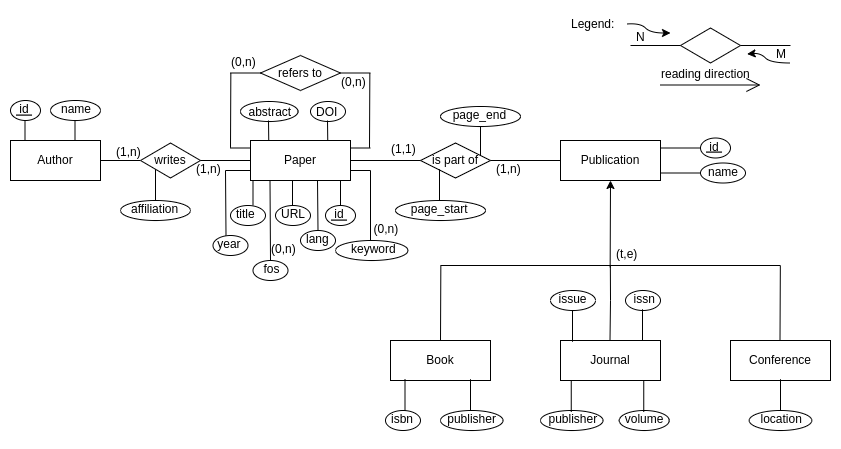
\includegraphics[width=0.9\textwidth]{Images/er}
        \caption{ER model of the bibliographic database.}
        \label{fig:er}%
    \end{center}
\end{figure}

\paragraph{More detailed description of entities}
\begin{itemize}
    \item \textbf{Paper}, as said before, is the most important entity, indeed it is in the middle of the model.
    Each paper is characterized by an ID, a title, a publication year, an abstract, a list of keywords, a list of fields of study, a DOI which is a unique global identifier, and a URL to reach the site where it is available for consultation.
    \item \textbf{Author} of a paper is identified by an ID and has a name, that contains both the name and the surname of the author.
    \item \textbf{Publication} is a total and exclusive hierarchy that represents the physical place where a paper is published, it has an ID and a name called the venue, and it is specialized in:
    \begin{itemize}
        \item \textbf{Conference} that has a location where it took place;
        \item \textbf{Book} that has a global identifier called ISBN and a publisher;
        \item \textbf{Journal} that has a global identifier called ISSN, a publisher,
        a volume and issue.
    \end{itemize}
\end{itemize}

\paragraph{More detailed description of relationships}
\begin{itemize}
    \item \textbf{WRITES} links Author and Paper, each author can write one or more papers, and each paper is written by one or more authors.
    This relationship has an attribute affiliation that is the organization the author was part of when the article was written.
    \item \textbf{REFERS TO} links two Paper entities, each paper can reference many papers and can be referenced by many papers.
    \item \textbf{IS PART OF} links Paper and Publication, each paper is published on a single publication and each publication can contain several papers.
    This relationship has as attributes the page\_start and page\_end of the article within the publication.
\end{itemize}

\paragraph{More detailed observations}
\begin{itemize}
    \item DOI could have been a good identifier for papers since it is globally unique, but in the used dataset not all articles had it.
    \item ORCiD is a unique identifier for authors that would have been a valid key for the entity Author but this data was not present in the used dataset.
    \item Since the focus is on the entity Paper and a simple model for the domain was built, it seemed not meaningful to have a separate entity to model the organization whose author is part of.
    In addition, that would have had just one attribute.
    For this reason, the concept of affiliation was modeled as an attribute of the relationship WRITES, storing multiple affiliations for the single author.
\end{itemize}
